\subsection*{Problema 22}

\textbf{Enunciado:}
Calcular la integral indefinida:
\begin{align*}
I = \int \dfrac{(1 - \cos x)\sin x}{\cos x + \cos^2 x} \, dx
\end{align*}

\textbf{Solución:}
Para resolver la integral dada, aplicamos el método de sustitución sugerido. Definimos la nueva variable:
\begin{align*}
u = \cos x, \quad du = -\sin x \, dx
\end{align*}
De esta forma, el término $\sin x \, dx$ se sustituye por $-du$. Reemplazando en la integral original, obtenemos:
\begin{align*}
I &= \int \dfrac{(1 - u)(-du)}{u + u^2} \\
I &= \int \dfrac{u - 1}{u(1 + u)} \, du
\end{align*}

Ahora, resolvemos la expresión racional resultante utilizando el método de fracciones parciales. Proponemos la siguiente descomposición:
\begin{align*}
\dfrac{u - 1}{u(1 + u)} = \dfrac{A}{u} + \dfrac{B}{1 + u}
\end{align*}

Multiplicando ambos lados por el denominador común $u(1 + u)$, obtenemos:
\begin{align*}
u - 1 = A(1 + u) + B u
\end{align*}

Para hallar los valores de las constantes $A$ y $B$, evaluamos en valores convenientes de $u$:
\begin{align*}
\text{Si } u = 0 &\implies -1 = A(1) \implies A = -1 \\
\text{Si } u = -1 &\implies -2 = B(-1) \implies B = 2
\end{align*}

Sustituyendo los valores de $A$ y $B$ en la integral, se tiene:
\begin{align*}
I &= \int \left( \dfrac{-1}{u} + \dfrac{2}{1 + u} \right) du
\end{align*}

Integramos cada término por separado:
\begin{align*}
I &= -\int \dfrac{1}{u} \, du + 2 \int \dfrac{1}{1 + u} \, du \\
I &= -\ln|u| + 2\ln|1 + u| + C
\end{align*}

Aplicando las propiedades de los logaritmos, podemos reescribir el resultado como:
\begin{align*}
I &= \ln|1 + u|^2 - \ln|u| + C \\
I &= \ln\left| \dfrac{(1 + u)^2}{u} \right| + C
\end{align*}

Finalmente, regresamos a la variable original $x$ sustituyendo $u = \cos x$:
\begin{align*}
I = \ln\left| \dfrac{(1 + \cos x)^2}{\cos x} \right| + C
\end{align*}

\begin{figure}[H]
	\centering
	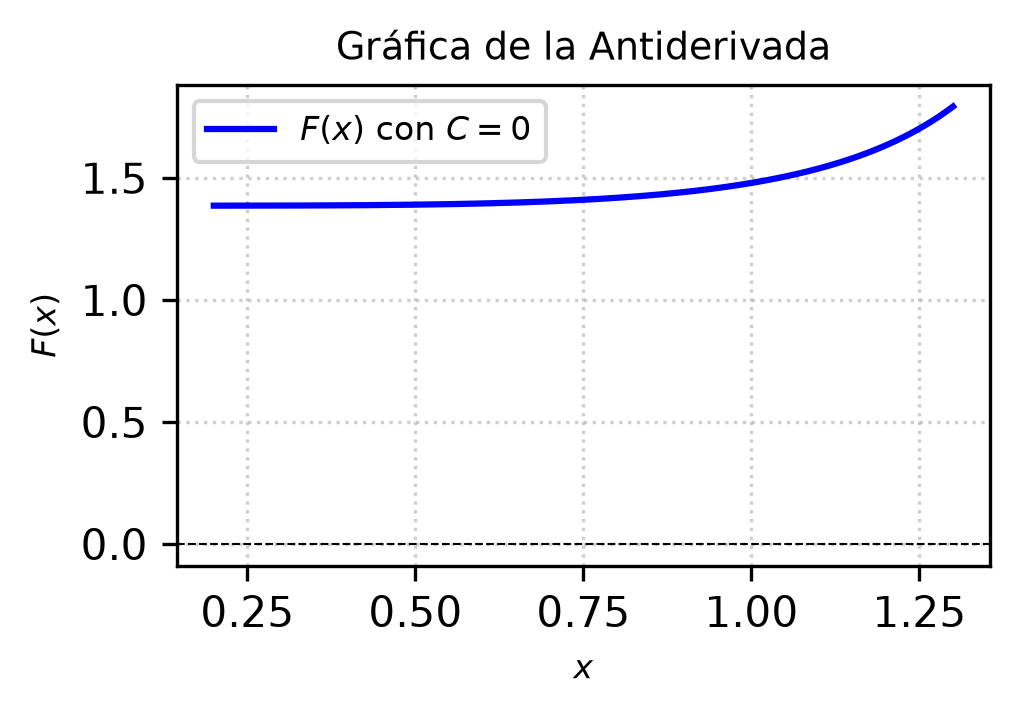
\includegraphics[width=\columnwidth]{semana_04/graficas/SEM04_P22_grafica.png}
	\caption{Representación gráfica de $f(x)$ y su antiderivada $F(x)$ evaluada para la constante de integración $C = 0$ (Problema 22).}
	\label{fig:problema22}
\end{figure}
